\documentclass[compress,trans,9pt]{beamer}
% \documentclass[9pt]{beamer}
%\documentclass[compress,9pt,usenames,dvipsnames]{beamer}
% \usepackage[utf8]{inputenc}
% \includeonlyframes{current}
\setbeamercovered{dynamic}
\usepackage{etex}
\usepackage{graphicx,url,psfrag}
\usepackage{tikz}
\usetikzlibrary{
  decorations.pathreplacing,
  calc,
  decorations.fractals,
  through,
  shapes,
  patterns,
  arrows.meta,
  decorations.pathreplacing,
  arrows,
  shapes,
  mindmap
}
\usepackage[center]{subfigure}
\usepackage{enumerate}
\usepackage[makeroom]{cancel}
\usepackage{mathtools}
\usepackage{graphbox}
\usepackage{amssymb}
% \usepackage[showframe]{geometry}
% \usepackage{enumitem}

%
% for warning sign
%
\usepackage{stackengine}
\usepackage{scalerel}
\usepackage{xcolor}
\newcommand\dangersign[1][2ex]{%
  \renewcommand\stacktype{L}%
  \scaleto{\stackon[1.3pt]{\color{red}$\triangle$}{\tiny !}}{#1}%
}
% %  The following is to show codes:
\usepackage{listings}
% \usepackage{color}
\usepackage{colortbl}
\usepackage{dbt}

\definecolor{dkgreen}{rgb}{0,0.6,0}
\definecolor{gray}{rgb}{0.5,0.5,0.5}
\definecolor{mauve}{rgb}{0.58,0,0.82}

% \definecolor{deepblue}{rgb}{0,0,0.5}
% \definecolor{deepred}{rgb}{0.6,0,0}
% \definecolor{deepgreen}{rgb}{0,0.5,0}
% \lstset{
%   language=Python,
%   backgroundcolor=\color{red},  % choose the background color. You must add \usepackage{color}
%   % backgroundcolor=\color{background},  % choose the background color. You must add \usepackage{color}
%   basicstyle=\footnotesize,
%   otherkeywords={self},
%   keywordstyle=\ttb\color{deepblue},
%   emph={MyClass,__init__},
%   emphstyle=\ttb\color{deepred},
%   stringstyle=\color{deepgreen},
%   commentstyle=\color{red},  %%%%%%%%
%   frame=tb,
%   showstringspaces=false
% }
%
% \lstdefinestyle{Python}{
%     language        = Python,
%     basicstyle      = \footnotesize,
%     keywordstyle    = \color{blue},
%     keywordstyle    = [2] \color{red}, % just to check that it works
%     stringstyle     = \color{green},
%     commentstyle    = \color{red}\ttfamily
% }

\lstset{frame=tb,
  language=Java,
  aboveskip=3mm,
  belowskip=3mm,
  showstringspaces=false,
  columns=flexible,
  basicstyle={\small\ttfamily},
  numbers=none,
  numberstyle=\tiny\color{gray},
  keywordstyle=\color{blue},
  commentstyle=\color{dkgreen},
  stringstyle=\color{mauve},
  breaklines=true,
  breakatwhitespace=true,
  tabsize=3
}
\lstset{language=Java}

\lstset{ %
  language=R,                     % the language of the code
  basicstyle=\footnotesize,       % the size of the fonts that are used for the code
  numbers=left,                   % where to put the line-numbers
  numberstyle=\tiny\color{gray},  % the style that is used for the line-numbers
  stepnumber=1,                   % the step between two line-numbers. If it's 1, each line
                                  % will be numbered
  numbersep=5pt,                  % how far the line-numbers are from the code
  backgroundcolor=\color{background},  % choose the background color. You must add \usepackage{color}
  showspaces=false,               % show spaces adding particular underscores
  showstringspaces=false,         % underline spaces within strings
  showtabs=false,                 % show tabs within strings adding particular underscores
  frame=single,                   % adds a frame around the code
  rulecolor=\color{black},        % if not set, the frame-color may be changed on line-breaks within not-black text (e.g. commens (green here))
  tabsize=2,                      % sets default tabsize to 2 spaces
  captionpos=b,                   % sets the caption-position to bottom
  breaklines=true,                % sets automatic line breaking
  breakatwhitespace=false,        % sets if automatic breaks should only happen at whitespace
  title=\lstname,                 % show the filename of files included with \lstinputlisting;
                                  % also try caption instead of title
  keywordstyle=\color{blue},      % keyword style
  commentstyle=\color{dkgreen},   % comment style
  stringstyle=\color{mauve},      % string literal style
  escapeinside={\%*}{*)},         % if you want to add a comment within your code
  morekeywords={*,...}            % if you want to add more keywords to the set
}
% \usepackage[usenames,dvipsnames]{color}
% \lstset{
%   language=Python,                     % the language of the code
%   basicstyle=\footnotesize,       % the size of the fonts that are used for the code
%   numbers=left,                   % where to put the line-numbers
%   numberstyle=\tiny\color{gray},  % the style that is used for the line-numbers
%   stepnumber=1,                   % the step between two line-numbers. If it's 1, each line
%                                   % will be numbered
%   numbersep=5pt,                  % how far the line-numbers are from the code
%   backgroundcolor=\color{background},  % choose the background color. You must add \usepackage{color}
%   showspaces=false,               % show spaces adding particular underscores
%   showstringspaces=false,         % underline spaces within strings
%   showtabs=false,                 % show tabs within strings adding particular underscores
%   frame=single,                   % adds a frame around the code
%   rulecolor=\color{black},        % if not set, the frame-color may be changed on line-breaks within not-black text (e.g. commens (green here))
%   tabsize=2,                      % sets default tabsize to 2 spaces
%   captionpos=b,                   % sets the caption-position to bottom
%   breaklines=true,                % sets automatic line breaking
%   breakatwhitespace=false,        % sets if automatic breaks should only happen at whitespace
%   title=\lstname,                 % show the filename of files included with \lstinputlisting;
%                                   % also try caption instead of title
%   keywordstyle=\ttb\color{blue},      % keyword style
%   commentstyle=\color{dkgreen},   % comment style
%   stringstyle=\color{mauve},      % string literal style
%   escapeinside={\%*}{*)},         % if you want to add a comment within your code
%   morekeywords={*,...}            % if you want to add more keywords to the set
% }

% \usepackage[dvipsnames]{xcolor}
% \newcommand{\Cross}{\mathbin{\tikz [x=1.4ex,y=1.4ex,line width=.2ex] \draw (0,0) -- (1,1) (0,1) -- (1,0);}}%
\newcommand{\Crossme}[1]{\!\!
\tikz [black,x=1.1em,y=1.1em,line width=.4ex]
\draw (-0.5,-0.5) -- (0,0) node {\footnotesize #1} -- (0.5,0.5) (0.5,-0.5) -- (-0.5,0.5);}%
\newcommand{\Checkme}[1]{\!\!
\tikz [x=1.1em,y=1.1em,line width=.4ex]
\draw [black] (0,0.7) -- (0.3,0) --(0.9,1.0) (0.5,0.5) node {\footnotesize #1};}
% \beamerdefaultoverlayspecification{<+-| alert@+>} %(this will show line by line)
\beamerdefaultoverlayspecification{<+->} %(this will show line by

% \usepackage{natbib}
% \input{../myMathSymbols.tex}
% \newcommand{\tlMr}[4]{\:{}^{\hspace{0.2em}#1}_{#2} \hspace{-0.1em}#3_{#4}}

% Smiley face\Smiley{} \Frowny{}
\usepackage{marvosym}
% -------------------------------------------------
%  Set directory for figs
% -------------------------------------------------
\usepackage{grffile}
\graphicspath{{Codes/}}
% -------------------------------------------------
%  Define colors
% -------------------------------------------------
\def\refcolor{cyan}
\newcommand{\myref}[1]{\small {\em #1}}
\def\excolor{brown}
% \usepackage{color}
% \usepackage[dvipsnames]{xcolor}


% % % Define danger sign
\newcommand*{\TakeFourierOrnament}[1]{{%
\fontencoding{U}\fontfamily{futs}\selectfont\char#1}}
\newcommand*{\danger}{\TakeFourierOrnament{66}}


% -------------------------------------------------
%  Define short-hand symbols.
% -------------------------------------------------
\newcommand{\B}{\textbf{B}}
\newcommand{\PP}{\mathbb{P}}
\newcommand{\E}{\mathbb{E}}
\newcommand{\D}{\mathbb{D}}
\newcommand{\W}{\dot{W}}
\newcommand{\ud}{\ensuremath{\mathrm{d}}}
\newcommand{\Ceil}[1]{\left\lceil #1 \right\rceil}
\newcommand{\Floor}[1]{\left\lfloor #1 \right\rfloor}
\newcommand{\sgn}{\text{sgn}}
\newcommand{\Lad}{\text{L}_{\text{ad}}^2}
\newcommand{\SI}[1]{\mathcal{I}\left[#1 \right]}
\newcommand{\SIB}[2]{\mathcal{I}_{#2}\left[#1 \right]}
\newcommand{\Indt}[1]{1_{\left\{#1 \right\}}}
\newcommand{\LadInPrd}[1]{\left\langle #1 \right\rangle_{\text{L}_\text{ad}^2}}
\newcommand{\LadNorm}[1]{\left|\left|  #1 \right|\right|_{\text{L}_\text{ad}^2}}
\newcommand{\Norm}[1]{\left|\left|  #1   \right|\right|}
\newcommand{\Ito}{It\^{o} }
\newcommand{\Itos}{It\^{o}'s }
\newcommand{\spt}[1]{\text{supp}\left(#1\right)}
\newcommand{\InPrd}[1]{\left\langle #1 \right\rangle}
\newcommand{\mr}{\textbf{r}}
\newcommand{\Ei}{\text{Ei}}
\newcommand{\arctanh}{\operatorname{arctanh}}
\newcommand{\ind}[1]{\mathbb{I}_{\left\{ {#1} \right\} }}
\newcommand{\Var}{\text{Var}}
\newcommand{\Cov}{\text{Cov}}
\newcommand{\Corr}{\text{Corr}}

\newcommand{\baseurl}[1]{\footnotesize\url{http://math.emory.edu/~lchen41/teaching/2020_Spring/#1}}


\newcommand*\mystrut[1]{\vrule width0pt height0pt depth#1\relax} % adding vertical space

\DeclareMathOperator{\esssup}{\ensuremath{ess\,sup}}

\newcommand{\steps}[1]{\vskip 0.3cm \textbf{#1}}
\newcommand{\calB}{\mathcal{B}}
\newcommand{\calC}{\mathcal{C}}
\newcommand{\calD}{\mathcal{D}}
\newcommand{\calE}{\mathcal{E}}
\newcommand{\calF}{\mathcal{F}}
\newcommand{\calG}{\mathcal{G}}
\newcommand{\calK}{\mathcal{K}}
\newcommand{\calH}{\mathcal{H}}
\newcommand{\calI}{\mathcal{I}}
\newcommand{\calL}{\mathcal{L}}
\newcommand{\calM}{\mathcal{M}}
\newcommand{\calN}{\mathcal{N}}
\newcommand{\calO}{\mathcal{O}}
\newcommand{\calT}{\mathcal{T}}
\newcommand{\calP}{\mathcal{P}}
\newcommand{\calR}{\mathcal{R}}
\newcommand{\calS}{\mathcal{S}}
\newcommand{\calV}{\mathcal{V}}
\newcommand{\bbC}{\mathbb{C}}
\newcommand{\bbN}{\mathbb{N}}
\newcommand{\bbP}{\mathbb{P}}
\newcommand{\bbZ}{\mathbb{Z}}
\newcommand{\myVec}[1]{\overrightarrow{#1}}
\newcommand{\sincos}{\begin{array}{c} \cos \\ \sin \end{array}\!\!}
\newcommand{\CvBc}[1]{\left\{\:#1\:\right\}}
\newcommand*{\one}{{{\rm 1\mkern-1.5mu}\!{\rm I}}}

\newcommand{\OneFrame}[1]{
\begin{enumerate}\item[#1] \phantom{av} \\[20em]\vfill\phantom{av}\myEnd\end{enumerate}}

\newcommand{\bH}{\ensuremath{\mathrm{H}}}
\newcommand{\Ai}{\ensuremath{\mathrm{Ai}}}

\newcommand{\R}{\mathbb{R}}
\newcommand{\myEnd}{\hfill$\square$}
\newcommand{\myQED}{\hfill\textcolor{lgtblue}{$\blacksquare$}}
\newcommand{\ds}{\displaystyle}
\newcommand{\Shi}{\text{Shi}}
\newcommand{\Chi}{\text{Chi}}
\newcommand{\Erf}{\ensuremath{\mathrm{erf}}}
\newcommand{\Erfc}{\ensuremath{\mathrm{erfc}}}
\newcommand{\He}{\ensuremath{\mathrm{He}}}
\newcommand{\Res}{\ensuremath{\mathrm{Res}}}

\newcommand{\mySeparateLine}{\begin{center}
 \makebox[\linewidth]{\rule{0.6\paperwidth}{0.4pt}}
\end{center}}

\theoremstyle{definition}
% \newtheorem{definition}[theorem]{Definition}
% \newtheorem{hypothesis}[theorem]{Hypothesis}
\newtheorem{assumption}[theorem]{Assumption}

\theoremstyle{plain}
% \newtheorem{theorem}{Theorem}
% \newtheorem{corollary}[theorem]{Corollary}
% \newtheorem{lemma}[theorem]{Lemma}
\newtheorem{proposition}[theorem]{Proposition}

\mode<presentation>
{
%      \usetheme{Warsaw}
%     \usetheme{JuanLesPins}
%  \usetheme{Hannover}
%  \usetheme{Montpellier}
   \useoutertheme{default}
  % or ...

  \setbeamercovered{transparent}
  % or whatever (possibly just delete it)
 \setbeamertemplate{frametitle}{
  \begin{centering}
    \color{blue}
    {\insertframetitle}
    \par
  \end{centering}
  }
}
\usefoottemplate{\hfill \insertframenumber{}}
% \inserttotalframenumber

\usepackage[english]{babel}
% or whatever

% \usepackage[latin1]{inputenc}
% or whatever

\usepackage{times}
\usepackage[T1]{fontenc}
% Or whatever. Note that the encoding and the font should match. If T1
% does not look nice, try deleting the line with the fontenc.

% \DeclareMathOperator{\Lip}{Lip}
\DeclareMathOperator{\lip}{l}
% \DeclareMathOperator{\Vip}{\overline{v}}
% \DeclareMathOperator{\vip}{\underline{v}}
% \DeclareMathOperator{\vv}{v}
% \DeclareMathOperator{\BC}{BC}
% \DeclareMathOperator{\CH}{CD}

\usepackage{pgfpages}
% \setbeameroption{show notes}
% \setbeamertemplate{note page}[plain]
% \setbeameroption{second mode text on second screen=right}
% \setbeameroption{show notes on second screen=right}
%
\title % (optional, use only with long paper titles)
{
Math 362: Mathematical Statistics II
}

% \subtitle
% {Research Plan} % (optional)

\author{Le Chen\\
\url{le.chen@emory.edu}\\
\url{chenle02@gmail.com}\\[2em]
Emory University\\
Atlanta, GA\\[2em]
\textcolor{gray}{\small Last updated on Spring 2021}\\
\textcolor{gray}{\small Last compiled on \today}
}
\institute[Emory University]
{%
\vspace{3em}
% \pgfuseimage{UNLV}
 }
 \vfill
% - Use the \inst command only if there are several affiliations.
% - Keep it simple, no one is interested in your street address.

% \date[Talk at Karlsruhe] % (optional)
% {\today }
 \date[Columbus]{
   2021 Spring\\[1em]
   Creative Commons License\\
   (CC By-NC-SA)
 }

\subject{}
% This is only inserted into the PDF information catalog. Can be left
% out.

% If you have a file called "university-logo-filename.xxx", where xxx
% is a graphic format that can be processed by latex or pdflatex,
% resp., then you can add a logo as follows:

% \pgfdeclareimage[height=0.8cm]{UNLV}{figs/UNLV-186.png}

% Delete this, if you do not want the table of contents to pop up at
% the beginning of each subsection:
% \AtBeginSubsection[]
% {
%   \begin{frame}<beamer>{Outline}
%     \tableofcontents[currentsection,currentsubsection]
%   \end{frame}
% }


% If you wish to uncover everything in a step-wise fashion, uncomment
% the following command:

% \beamerdefaultoverlayspecification{<+->}
% % % % % % % % % % % % % % % % % % %
%  Define a block
% % % % % % % % % % % % % % % % % % %
\newenvironment<>{problock}[1]{%
  \begin{actionenv}#2%
      \def\insertblocktitle{#1}%
      \par%
      \mode<presentation>{%
        \setbeamercolor{block title}{fg=white,bg=olive!95!black}
       \setbeamercolor{block body}{fg=black,bg=olive!25!white}
       \setbeamercolor{itemize item}{fg=white!20!white}
       \setbeamertemplate{itemize item}[triangle]
     }%
      \usebeamertemplate{block begin}}
    {\par\usebeamertemplate{block end}\end{actionenv}}

\newenvironment<>{assblock}[1]{%
  \begin{actionenv}#2%
      \def\insertblocktitle{#1}%
      \par%
      \mode<presentation>{%
        \setbeamercolor{block title}{fg=white,bg=green!50!black}
       \setbeamercolor{block body}{fg=black,bg=green!10}
       \setbeamercolor{itemize item}{fg=green!80!black}
       \setbeamertemplate{itemize item}[triangle]
     }%
      \usebeamertemplate{block begin}}
    {\par\usebeamertemplate{block end}\end{actionenv}}


\newcommand{\mySection}[1]{\section{\S\: #1}\begin{frame}{\myChapter}\tableofcontents[currentsection]\end{frame}}

\AtBeginSection[]
  {
     \begin{frame}<beamer>
     \frametitle{Plan}
     \tableofcontents[currentsection]
     \end{frame}
  }


\begin{document}

\AtBeginSection[]
  {
     \begin{frame}<beamer>
     \frametitle{Plan}
     \tableofcontents[currentsection]
     \end{frame}
  }


%-------------- start slide -------------------------------%{{{
\begin{frame}[noframenumbering]
  \titlepage
\end{frame}
%-------------- end slide -------------------------------%}}}


% \begin{frame}{Outline}
%   \tableofcontents
%   % You might wish to add the option [pausesections]
% \end{frame}


\newcommand{\myChapter}{Chapter 10. Goodness-of-fit Tests}
%-------------- start slide -------------------------------%{{{
\begin{frame}
\begin{center}
\huge
\myChapter
\end{center}
\end{frame}
%-------------- end slide -------------------------------%}}}
\mySection{10.1 Introduction}
%-------------- start slide -------------------------------%{{{ 10.4
\begin{frame}
	\centering
	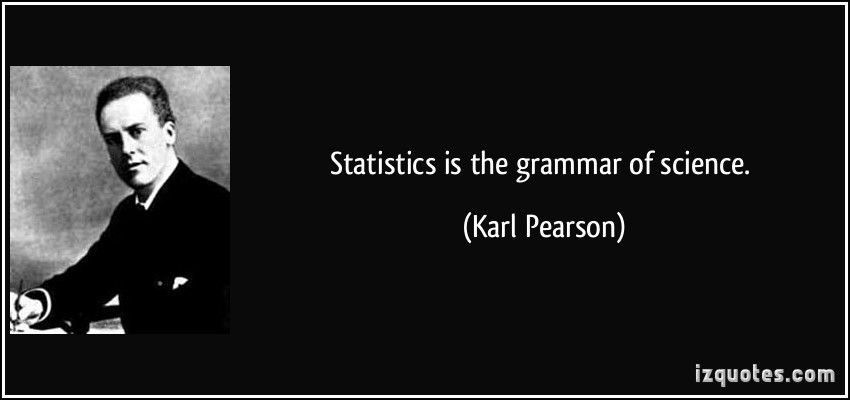
\includegraphics[scale=0.4]{Pearson_quote.jpg}
	\vfill
	\begin{enumerate}
		\item Karl Pearson, 1857 -- 1936.
		\item English mathematician and biostatistician.
		\item He has been credited with establishing the discipline of mathematical statistics
		\item Method of moments; p-Value; \underline{Chi-square test}; Foundations of statistical hypothesis testing theory; principle component analysis ...
	\end{enumerate}
\end{frame}
%-------------- end slide -------------------------------%}}}
%-------------- start slide -------------------------------%{{{ 10.5
\begin{frame}
\centering
Pearson's chi-squared test\\ in one shot
\vfill

\includegraphics[scale=0.15]{Goodness_fit_test_puzzle-neg.png}
\vfill
\[
	\chi^2 =\sum  \frac{ \left( \text{Observed} - \text{Expected} \right)^2 }{\text{Expected}} \sim \text{Chi Square of $df$}
\]
\vfill
\[
	df = \text{numer of classes} -\text{number of estimated parameters} - 1
\]
\vfill
All expected $\ge 5$
\end{frame}
%-------------- end slide -------------------------------%}}}

\mySection{10.2 The Multinomial Distribution}
%-------------- start slide -------------------------------%{{{ 10.8
\begin{frame}
	% {\S\: 10.2 The Multinomial Distribution}
	
\includegraphics[scale=0.5]{MM-neg.jpeg}
\begin{enumerate}
\item[Def.] Suppose one does an experiment of extracting $n$ balls of $t$ different colors from a jar,
	replacing the extracted ball after each draw.
	Balls from the same color are equivalent.
	Denote the variable which is the number of extracted balls of color $i$ ($i = 1, ..., t$) as $X_i$,
	and denote as $p_i$ the probability that a given extraction will be in color $i$.
	The probability distribution function of the vector $(X_1,\cdots,X_t)$ is called
	the \textcolor{yellow}{multinomial distribution}, which is equal to
	\begin{align*}
		p_{X_1,\cdots,X_t}(k_1,\cdots,k_t)
		&= \bbP\left( X_1=k_1,\cdots,X_t=k_t \right)\\
		&= {n\choose k_1,\cdots,k_t} p_1^{k_1}\cdots p_t^{k_t}
	\end{align*}
	where $k_i\in\{0,1,\cdots, n\}$, $1\le i\le t$, $\sum_{i=1}^t k_i=n$, and $p_1+\cdots+p_t=1$.
\end{enumerate}
\end{frame}
%-------------- end slide -------------------------------%}}}
%-------------- start slide -------------------------------%{{{ 10.9
\begin{frame}
	% {Properties of multinomial distribution}
	\begin{enumerate}
		\item[Thm] Suppose $(X_1,\cdots, X_t)$ follows the multinomial distribution with parameters $n$ and $(p_1,\cdots,p_t)$ with $p_i\ge 0$ and $\sum_{i}p_i=1$. Then\\[1em]
		\item $X_i\sim$Binomail($n,p_i$) and hence\\[2em]
		\item[] $\E[X_i] = n p_i$
		\item[] $\Var(X_i) = n p_i(1-p_i)$
		\vfill
		\item $\text{Cov}(X_i,X_j) = -np_ip_j$, $i\ne j$. \hfill (negative correlated)
		\vfill
		\item $M_{X_1,\cdots,X_t}(s_1,\cdots,s_t) = \left(p_1e^{s_1} + \cdots + p_t e^{s_t} \right)^n$.
	\end{enumerate}
\end{frame}
%-------------- end slide -------------------------------%}}}
%-------------- start slide -------------------------------%{{{ 10.10
\begin{frame}[fragile]

	\begin{enumerate}
		\item[Proof]
		\item[(3)]
\begin{align*}
	M_{X_1,\cdots,X_t}(s_1,\cdots,s_t) & = \E \left[e^{X_1 s_1+\cdots+X_t s_t} \right ]                                                                                        \\
                                     & = \mathop{\sum_{k_1,\cdots,k_t=0}^n}_{k_1+\cdots+k_t=n} {n\choose k_1,\cdots,k_t} p_1^{k_1}\cdots p_t^{k_t}e^{k_1 s_1+\cdots+k_t s_t} \\
                                     & = \mathop{\sum_{k_1,\cdots,k_t=0}^n}_{k_1+\cdots+k_t=n} {n\choose k_1,\cdots,k_t} (p_1e^{s_1})^{k_1}\cdots (p_te^{s_t})^{k_t}         \\
                                     & = \left(p_1e^{s_1}+\cdots+p_te^{s_t} \right)^n
\end{align*}
\vfill
\item[(1)] To find $M_{X_i}(s_i)$, we simply set $s_j\equiv 0$ for $j\ne i$. Hence
	\[
		M_{X_i}(s_i) = \big(\underbrace{p_1+\cdots+p_{i-1}+p_{i+1}+\cdots+p_t}_{=1-p_i}+p_ie^{s_i} \big)^n
		\:\Longrightarrow\:
		\text{$X_i\sim$ Binomial$(n,p_i)$}
	\]
	\end{enumerate}
\end{frame}
%-------------- end slide -------------------------------%}}}
%-------------- start slide -------------------------------%{{{ 10.11
\begin{frame}[fragile]

	\begin{enumerate}
		\item[(2)] Set $M:=M_{X_1,\cdots,X_t}(s_1,\cdots,s_t)$. Then for $i\ne j$,
		\item[]
			\begin{align*}
				\frac{\partial M}{\partial s_i} =n \left(p_1e^{s_1}+\cdots+p_te^{s_t} \right)^{n-1} p_i e^{s_i}
			\end{align*}
		\item[]
			\begin{align*}
				\frac{\partial^2 M}{\partial s_i\partial s_j} =n(n-1) \left(p_1e^{s_1}+\cdots+p_te^{s_t} \right)^{n-2} p_i e^{s_i}p_j e^{s_j}
			\end{align*}
		\item[]
			\[
			\Downarrow
			\]
			\[
		\E[X_iX_j] = \frac{\partial^2 M}{\partial s_i\partial s_j}\bigg|_{s_1=\cdots=s_t=0}= n(n-1)(p_1+\cdots+p_t)^{n-2}p_ip_j			=n(n-1)p_ip_j\]
	\item[]
		\[\Downarrow\]
		\begin{align*}
			\Cov(X_i,X_j)
		&= \E[X_iX_j] - \E[X_i]\E[X_j]
	      \\&= n(n-1)p_ip_j - np_i\times np_j \\
		&= - np_ip_j
		\end{align*}
		\myEnd
	\end{enumerate}
\end{frame}
%-------------- end slide -------------------------------%}}}
%-------------- start slide -------------------------------%{{{ 10.12
\begin{frame}

From a continuous pdf to a multinomial distribution:
\vfill
\begin{enumerate}
	\item[E.g.] Let $Y_i$ be a random sample of size $n$ from $f_Y(y)=6y(1-y)$, $y\in[0,1]$.
		Define
		\[
		X_i =
		\begin{cases}
			1 & Y_i \in [0,0.25)\\
			2 & Y_i \in [0.25,0.5)\\
			3 & Y_i \in [0.5,0.75)\\
			4 & Y_i \in [0.75,1)
		\end{cases}
		\]
		Find the distribution of $(X_1,\cdots,X_n)$.
		\vfill
	\item[Sol.] $(X_1,X_2,X_3,X_4)$ follows multinomial distribution with parameters $(p_1,p_2,p_3,p_4)$ where
		\begin{align*}
			p_1 = \int_0^{\frac{1}{4}}6y(1-y)dy = \cdots = \frac{5}{32},
		\end{align*}
\end{enumerate}
\end{frame}
%-------------- end slide -------------------------------%}}}
%-------------- start slide -------------------------------%{{{ 10.13
\begin{frame}
\centering
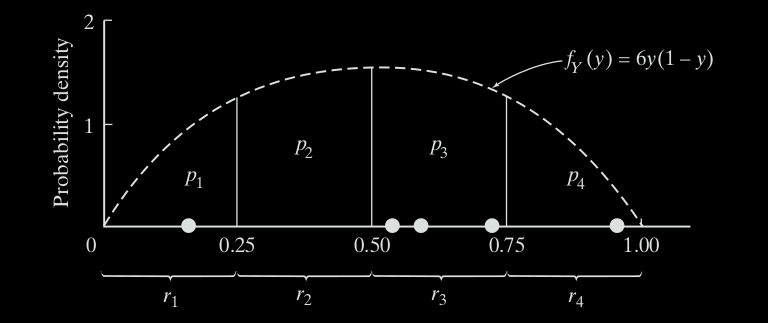
\includegraphics[scale=0.35]{Figure_10-2-2-neg.png}
\vfill
\begin{enumerate}
	\item[] and by symmetry,
		\begin{align*}
			 p_4=p_1=\frac{5}{32}\quad\text{and}\quad
			 p_2=p_3 = \frac{1}{2}\left(1-p_1-p_4\right) = \frac{11}{32}.
		\end{align*}
		\myEnd
		\bigskip
	\item[Remark] In this way, we transform the outcomes, any values between $[0,1]$, into \textcolor{yellow!80!black}{\bf categorical data}.
This chapter is about
\item[]
		\begin{center}
		\bf Analysis of Categorical Data
		\end{center}
\end{enumerate}
\end{frame}
%-------------- end slide -------------------------------%}}}

\mySection{10.3 Goodness-of-Fit Tests: All Parameters Known}
%-------------- start slide -------------------------------%{{{ 10.16
\begin{frame}
	% {\S\: 10.3 Goodness-of-Fit Tests: All Parameters Known}
	\begin{enumerate}
		\item[Rationale]
		\item[$!$] We want to test if the c.d.f. $F_Y(\cdot)$ is given by the true c.d.f. $F_0(\cdot)$, i.e., \\[1em]
			\[H_0:F_Y(y) = F_0(y)\quad v.s. \quad H_1: F_Y(y)\ne F_0(y)
			\]
			\vfill
		\item[$\sim$] By properly partitioning the domain, the random sample should follow
		\begin{center}
			\textcolor{yellow!80!black}{\it an induced multinomial distribution}.
		\end{center}
		\vfill
		\item[$\Longrightarrow$] Then testing $F_Y(\cdot)=F_0(\cdot)$ reduces to testing the induced multinomial distribution of the following form: \\[1em]
			\[
			H_0: p_1 = p_1', \cdots, p_n =p_n'
			\]
			\[
			v.s.
			\]
			\[
				H_1: p_i\ne p_i'\quad\text{for at least one $i$}
			\]
	\end{enumerate}
\end{frame}
%-------------- end slide -------------------------------%}}}
%-------------- start slide -------------------------------%{{{ 10.17
\begin{frame}[fragile]

	\begin{enumerate}
		\item[How]
		\item Suppose we are sampling from the c.d.f. $F(y)$
			\vfill
		\item Divide the range of the distribution into $k$ mutually exclusive and exhausive intervals, say $I_1,\cdots, I_k$.
			\vfill
		\item Let $\pi_i = \bbP(X\in I_i)$, $i=1,\cdots, k$.
			\vfill
		\item Let $O_1,\cdots,O_k$ be the respective
			observed numbers of the observations $X_1,\cdots, X_n$ in
			the intervals $I_1,\cdots,I_k$.
			\vfill
		\item Then $O=(O_1,\cdots,O_k)\sim $ multinomial distribution with $(\pi_1,\cdots,\pi_k)$, i.e.,
			\[
				\bbP\left(O_1=o_1,\cdots, O_k=o_k \right )
				=\frac{n!}{\prod_{i=1}^k o_i!}\prod_{i=1}^k \pi_i^{o_i}
			\]
			with  $\sum_{i=1}^k \pi_i=1$, $\sum_{i=1}^k o_i = n$, and
			\[
				\E[O_i] = n\pi_i =:e_i, \quad \Var(O_i) = n \pi_i(1-\pi_i)
			\]
	\end{enumerate}
\end{frame}
%-------------- end slide -------------------------------%}}}
%-------------- start slide -------------------------------%{{{ 10.18
\begin{frame}[fragile]

	\begin{enumerate}
		\setcounter{enumi}{5}
		\item When $k=2$, by CLT,  as $n\rightarrow \infty$,
			\[
				\frac{O_1-n\pi_1}{\sqrt{n\pi_1(1-\pi_1)}}\stackrel{d}{\rightarrow} N(0,1)\quad
				\Longrightarrow\quad
				\frac{(O_1-n\pi_1)^2}{n\pi_1(1-\pi_1)}\stackrel{d}{\rightarrow}\chi^2_1
			\]
		\item[]
				\[\hspace{12em}||\]
			\[
\hspace{12em}\frac{(O_1-n\pi_1)^2}{n\pi_1}
+\frac{(O_2-n\pi_2)^2}{n\pi_2}
			\]
		\item[]
			\[\hspace{12em}||\]
			\[
				\hspace{12em}\frac{(O_1-e_1)^2}{e_1}
				+\frac{(O_2-e_2)^2}{e_2}
			\]
			\vfill
		\item[] Hence, as $n\to\infty$,
			\[
				\sum_{i=1}^k
				\frac{(O_i-e_i)^2}{e_i}\stackrel{d}{\rightarrow}\chi^2_{k-1}
			\]
	\end{enumerate}
\end{frame}
%-------------- end slide -------------------------------%}}}
%-------------- start slide -------------------------------%{{{ 10.19
\begin{frame}[fragile]

	\begin{enumerate}
		\setcounter{enumi}{6}
\item For general $k$,
			\[
\sum_{i=1}^k
\frac{(O_i-n\pi_i)^2}{n\pi_i} =
\sum_{i=1}^k
\frac{(O_i-e_i)^2}{e_i}
			\]
			follows a complicated, but exact, distribution, from which, one can show
			\[
	\sum_{i=1}^k
\frac{(O_i-e_i)^2}{e_i} \stackrel{d}{\rightarrow}\chi^2_{k-1}
			\]
			\vfill
		\item[]
			\[\Downarrow\]
			\vfill
		\item[Thm.] When $n$ is large enough, namely, when $n\pi_i\ge 5$ for all $i$,
			\[
				D=	\sum_{i=1}^k
				\frac{(O_i-e_i)^2}{e_i} \stackrel{appr.}{\sim}\chi^2_{k-1}.
			\]
			\vfill
		\item[Rmk:] The above is called {\em Pearson's chi-square test}. It is asymptotically equivalent to the generalized likelihood ratio test.
	\end{enumerate}
\end{frame}
%-------------- end slide -------------------------------%}}}
%-------------- start slide -------------------------------%{{{ 10.20
\begin{frame}[fragile]{Alternative: G-test\\
	\small -- the likelihood ration test for multinomial model}

	\begin{enumerate}
		\item Under $H_0:\pi_i=p_i$, $i=1,\cdots,k$, the MLE of $\pi_i$ are
			\[
				\widetilde\pi_i = p_i =  \frac{np_i}{n} =  \frac{e_i}{n},\qquad \forall i.
			\]
			\vfill
		\item When there are no constraints, for $i=1,\cdots,k-1$,
			\[
				\frac{\partial}{\partial \pi_i} \ln L(\pi_1,\cdots,\pi_{k-1}|o_1,\cdots,o_k)  = 0  ,\quad 1\le i\le k-1
			\]
			\[\text{\rotatebox[origin=c]{90}{$\Leftrightarrow$}}\]
			\[
				\frac{o_i}{\widehat\pi_i} = \frac{o_k}{1-\widehat\pi_1-\cdots - \widehat\pi_{k-1}},\quad 1\le i\le k-1
			\]
			\[\text{\rotatebox[origin=c]{90}{$\Leftrightarrow$}}\]
			\[
				\widehat\pi_i = \frac{o_i}{n},\quad 1\le i\le k.
			\]
	\end{enumerate}
\end{frame}
%-------------- end slide -------------------------------%}}}
%-------------- start slide -------------------------------%{{{ 10.21
\begin{frame}[fragile]

	\begin{enumerate}
		\setcounter{enumi}{3}
	\item[$\Rightarrow$]
		\begin{align*}
			\lambda := \ln \left( \frac{L(\widetilde\pi_1,\cdots,\widetilde\pi_{k-1}|o_1,\cdots,o_k)}{L(\widehat\pi_1,\cdots,\widehat\pi_{k-1}|o_1,\cdots,o_k)} \right)
			&= \log \left( \frac{\prod_{i=1}^k \widetilde{\pi}_i^{o_i}}{\prod_{i=1}^k \widehat{\pi}_i^{o_i}}\right)\\
			\\&=\sum_{i=1}^k o_i \ln \left(  \frac{\widetilde\pi_i}{\widehat\pi_i}\right )
			\\&=\sum_{i=1}^k o_i \ln \left(  \frac{e_i}{o_i}\right )
		\end{align*}
	\item[] Critical region: $\lambda<\lambda_*<0$.
		\vfill
	\item[Def.]
		\[
			G: = -2 \lambda = -2\sum_{i=1}^k o_i \ln \left(  \frac{e_i}{o_i}\right )
=2\sum_{i=1}^k o_i \ln \left(  \frac{o_i}{e_i}\right )
		\]
	\item[] $G \stackrel{approx.}{\sim} \chi^2_{k-1}$ for large $n$.
	\item[] Critical region: $G\ge G_* = \chi^2_{1-\alpha,k-1}$.
\end{enumerate}
\end{frame}
%-------------- end slide -------------------------------%}}}
%-------------- start slide -------------------------------%{{{ 10.22
\begin{frame}[fragile]

	\begin{enumerate}
		\item[Relation] G-test and Pearson's Chi square test
			\vfill
		\item[] By second order Taylor expanson around $1$,
			\begin{align*}
				G &= -2 \sum_{i=1}^k o_i \ln \left(  \frac{e_i}{o_i}\right )\\
				  &\approx
				  -2\sum_{i=1}^k o_i \left[ \left( \frac{e_i}{o_i} -1\right )-\frac12 \left(\frac{e_i}{o_i}-1 \right )^2  \right ]
				\\&=
				-2\sum_{i=1}^k (e_i-o_i) + \sum_{i=1}^k o_i\left(\left(1-\frac{o_i}{e_i}\right)+\frac{o_i}{e_i} \right)\left(\frac{e_i}{o_i}-1 \right )^2
				\\& = 0 + \sum_{i=1}^n \frac{o_i^2}{e_i} \left(1-\frac{o_i}{e_i} \right)^3 +  \sum_{i=1}^k \frac{(e_i-o_i)^2}{e_i}
				\\& \approx \sum_{i=1}^k \frac{(e_i-o_i)^2}{e_i}
			\end{align*}
		\item[]
			\vspace{-1em}
			\begin{minipage}{0.5\textwidth}
			\[||\]
			\[D\]
			\end{minipage}
			\vfill
		\item[$\therefore$] Pearson's Chi-square test is an approximation of G-test.
	\end{enumerate}
\end{frame}
%-------------- end slide -------------------------------%}}}
%-------------- start slide -------------------------------%{{{ 10.23
\begin{frame}
\begin{enumerate}
\item[E.g. 1] {\it Benford's law}:
\begin{center}
\begin{minipage}{0.5\textwidth}
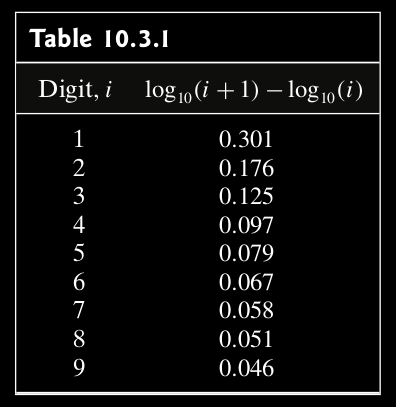
\includegraphics[scale=0.3]{Table_10-3-1-neg.png}
\end{minipage}
% \hspace{2em}
\begin{minipage}{0.333\textwidth}
Initial digits\\
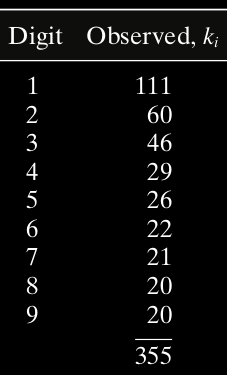
\includegraphics[scale=0.25]{Table_10-3-2-2-neg.png}
\end{minipage}
\end{center}
Use this law to check whether the bookkeepers have made up entries. \\[1em]
Assume that bookkeepers are not aware of Benford's law.
\end{enumerate}
\end{frame}
%-------------- end slide -------------------------------%}}}
%-------------- start slide -------------------------------%{{{ 10.24
\begin{frame}

\begin{enumerate}
\item[Sol.] The test should be
\begin{align*}
&H_0: p_1=p_{10},\cdots,p_9=p_{90}
\\& \hspace{4em} v.s.\\ &
H_1: p_i\ne p_{i0} \quad \text{for at least one $i=1,\cdots, 9$.}
\end{align*}
% \item[]
% \begin{center}
% 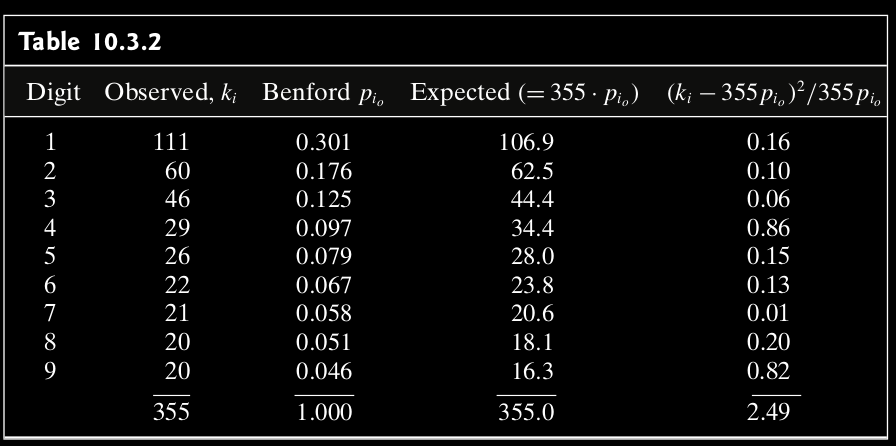
\includegraphics[scale=0.3]{Table_10-3-2-neg.png}
% \end{center}
\vfill
\item[] Critical region: $\left(\chi_{.95,8}^2,\infty \right)=(15.507,\infty)$.
\end{enumerate}
\end{frame}
%-------------- end slide -------------------------------%}}}
%-------------- start slide -------------------------------%{{{ 10.25
\begin{frame}[fragile]
		Compute the $D$ and $G$ scores:
		\vfill
			\begin{center}
				 \renewcommand{\arraystretch}{1.6}
				\begin{tabular}{ccc|ccc}
					\hline
			Digit & $o_i$ & $p_i$ & $e_i$ & $(o_i-e_i)^2/e_i$              & $2o_i\ln(e_i/o_i)$ \\ \hline
			1     & 111   & 0.301 &       &                                & \cr
			2     & 60    & 0.176 &       &                                & \cr
			3     & 46    & 0.125 &       &                                & \cr
			4     & 29    & 0.097 &       &                                & \cr
			5     & 26    & 0.079 &       &                                & \cr
			6     & 22    & 0.067 &       &                                & \cr
			7     & 21    & 0.058 &       &                                & \cr
			8     & 20    & 0.051 &       &                                & \cr
			9     & 20    & 0.046 &       &                                & \cr \hline
			sum   & 355   & 1     & 355   & $d=\underline{\phantom{aaaa}}$ & $g=\underline{\phantom{aaaa}}$ \cr \hline
	\end{tabular}
	\end{center}
\end{frame}
%-------------- end slide -------------------------------%}}}
%-------------- start slide -------------------------------%{{{ 10.26
\begin{frame}[fragile]
	\begin{center}
	\renewcommand{\arraystretch}{1.6}
		\begin{tabular}{ccc|ccc}
			\hline
			Digit & $o_i$ & $p_i$ & $e_i$ & $(o_i-e_i)^2/e_i$    & $2o_i\ln(e_i/o_i)$ \\ \hline
			1     & 111   & 0.301 & 106.9 & 0.16                 & 8.449\cr
			2     & 60    & 0.176 & 62.5  & 0.10                 & -4.860\cr
			3     & 46    & 0.125 & 44.4  & 0.06                 & 3.309\cr
			4     & 29    & 0.097 & 34.4  & 0.86                 & -9.963\cr
			5     & 26    & 0.079 & 28.0  & 0.15                 & -3.937\cr
			6     & 22    & 0.067 & 23.8  & 0.13                 & -3.433\cr
			7     & 21    & 0.058 & 20.6  & 0.01                 & 0.828\cr
			8     & 20    & 0.051 & 18.1  & 0.20                 & 3.982\cr
			9     & 20    & 0.046 & 16.3  & 0.82                 & 8.109\cr \hline
			sum   & 355   & 1     & 355   & $d=\underline{2.49}$ & $g=\underline{2.48}$\cr\hline
		\end{tabular}
	\vfill
	Conclusion: Fail to reject.
	\end{center}
\end{frame}
%-------------- end slide -------------------------------%}}}
%-------------- start slide -------------------------------%{{{ 10.27
\begin{frame}[fragile]
	\begin{center}
	\begin{lstlisting}
> #  EX 10.3.2
> library(data.table)
> mydat <- fread('http://math.emory.edu/~lchen41/teaching/2020_Spring/Case_10-3-2.data')
trying URL 'http://math.emory.edu/~lchen41/teaching/2020_Spring/Case_10-3-2.data'
Content type 'unknown' length 153 bytes
==================================================
downloaded 153 bytes

> head(mydat)
   Digit  Oi    Pi
1:     1 111 0.301
2:     2  60 0.176
3:     3  46 0.125
4:     4  29 0.097
> pi = mydat[,3]
> oi = mydat[,2]
> n = sum(oi)
> ei = n*pi
> di = (ei-oi)^2/ei
> gi =  2*oi*log(oi/ei)
> print(paste("Using Pearson's test, D value is equal to ", round(sum(di),3)))
[1] "Using Pearson's test, D value is equal to  2.491"
> print(paste("Using the G-test, G value is equal to ", round(sum(gi),3)))
[1] "Using the G-test, G value is equal to  2.484"
	\end{lstlisting}
\footnotesize
Codes available
\\
\baseurl{Case_10-3-2.R}
	\end{center}
\end{frame}
%-------------- end slide -------------------------------%}}}
%-------------- start slide -------------------------------%{{{ 10.28
\begin{frame}
\begin{enumerate}
\item[E.g. 2] Test for randomness\\[1em]
Is the following sample of size $40$ from $f_Y(y)=6y(1-y)$, $y\in[0,1]$?
\vfill
\begin{center}
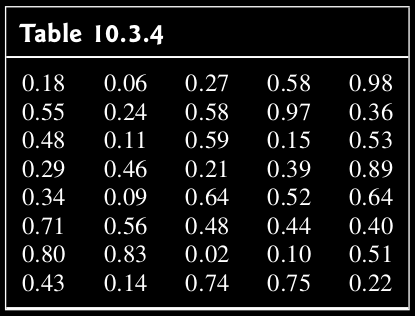
\includegraphics[scale=0.3]{Table_10-3-4-neg.png}
\end{center}
\end{enumerate}
\end{frame}
%-------------- end slide -------------------------------%}}}
%-------------- start slide -------------------------------%{{{ 10.29
\begin{frame}

\begin{enumerate}
\item[Sol.] Test continuous pdf $\rightarrow$ reduce to a set of classes:
\begin{center}
% 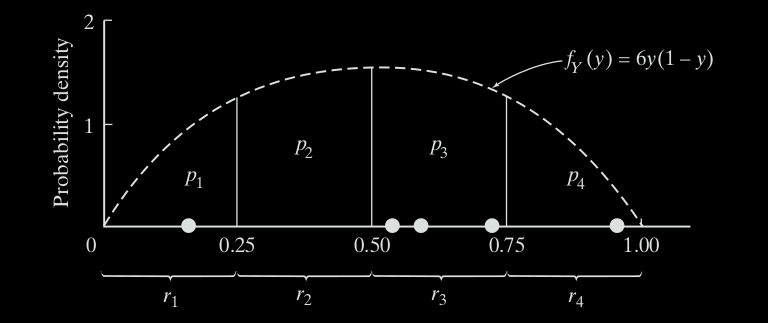
\includegraphics[scale=0.18]{Figure_10-2-2-neg.png}	\\ \pause
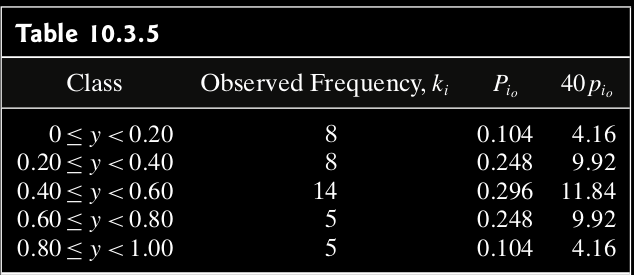
\includegraphics[scale=0.25]{Table_10-3-5-neg.png}\\ \pause
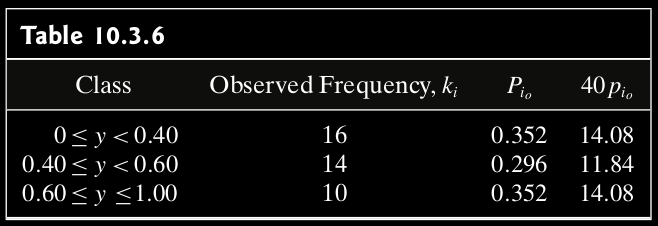
\includegraphics[scale=0.24444]{Table_10-3-6-neg.png} \pause
\end{center}
\[
d = \cdots =1.84.
\]
\item[] Critical region: $\left(\chi_{.95,2}^2,\infty \right)=(5.992,\infty)$.
\item[] Conclusion: Fail to reject.
\end{enumerate}
\end{frame}
%-------------- end slide -------------------------------%}}}
%-------------- start slide -------------------------------%{{{ 10.30
\begin{frame}[fragile]
	\begin{lstlisting}
> # Case Study 10.3.2
> # Read data from the URL link
> library(data.table)
> mydat <- fread('http://math.emory.edu/~lchen41/teaching/2020_Spring/EX_10-3-1.data')
trying URL 'http://math.emory.edu/~lchen41/teaching/2020_Spring/EX_10-3-1.data'
Content type 'unknown' length 234 bytes
==================================================
downloaded 234 bytes

>d(mydat)
   Col1 Col2 Col3 Col4 Col5
   1: 0.18 0.06 0.27 0.58 0.98
   2: 0.55 0.24 0.58 0.97 0.36
   3: 0.48 0.11 0.59 0.15 0.53
   4: 0.29 0.46 0.21 0.39 0.89
   5: 0.34 0.09 0.64 0.52 0.64
   6: 0.71 0.56 0.48 0.44 0.40
# Conditions for lower bounds
> lb=c(0,0.40,0.60)
> # Conditions for upper bounds
> up=c(0.40,0.60,1.00)
> # Store the results in d
> oi <- seq(1:length(lb))
> pi <- seq(1:length(lb))
> integrand <- function(y) {6*y*(1-y)}
> for (i in c(1:length(lb))) {
+   oi[i] <- table(mydat>=lb[i] & mydat<up[i])[2]
+   pi[i] <- integrate(integrand,  lb[i], up[i])$value[1]
+   print(paste("the", i,"th bin has", oi[i],
+       "entries and pi is equal to", pi[i]))
+ }
	\end{lstlisting}
\end{frame}
%-------------- end slide -------------------------------%}}}
%-------------- start slide -------------------------------%{{{ 10.31
\begin{frame}[fragile]
\begin{center}
\begin{minipage}{0.8\textwidth}
\begin{lstlisting}
[1] "the 1 th bin has 16 entries and pi is equal to 0.352"
[1] "the 2 th bin has 14 entries and pi is equal to 0.296"
[1] "the 3 th bin has 10 entries and pi is equal to 0.352"
> pi <- unlist(pi)
> n <- sum(oi)
> ei <- n*pi
> di <- (ei-oi)^2/ei
> gi <-  2*oi*log(oi/ei)
> rbind(oi,pi,ei,di,gi)
         [,1]       [,2]      [,3]
oi 16.0000000 14.0000000 10.000000
pi  0.3520000  0.2960000  0.352000
ei 14.0800000 11.8400000 14.080000
di  0.2618182  0.3940541  1.182273
gi  4.0906679  4.6920636 -6.843405
> print(paste("Using Pearson's test, D value is equal to ",round(sum(di),3)))
[1] "Using Pearson's test, D value is equal to  1.838"
> print(paste("Using the G-test, G value is equal to ", round(sum(gi),3)))
[1] "Using the G-test, G value is equal to  1.939"<Paste>
\end{lstlisting}
\end{minipage}
\vfill
\baseurl{EX_10-3-1.R}
\end{center}
\end{frame}
%-------------- end slide -------------------------------%}}}
%-------------- start slide -------------------------------%{{{ 10.32
\begin{frame}

\begin{enumerate}
\item[E.g. 3] Fisher's suspicion on Mendel's experiments on 1866:
\\
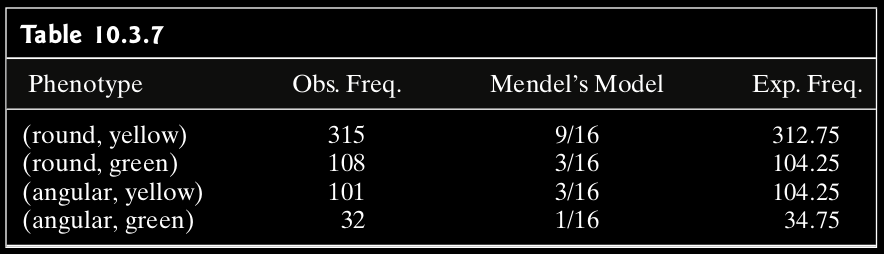
\includegraphics[scale=0.3]{Table_10-3-7-neg.png}
\vfill
\[
d= ... = 0.47
\]
\vfill
\[
P\text{-value} = \bbP(\chi_{3}^2 \le 0.47) = 0.0746.
\]
\end{enumerate}
\end{frame}
%-------------- end slide -------------------------------%}}}
%-------------- start slide -------------------------------%{{{ 10.33
\begin{frame}[fragile]

\begin{minipage}{0.4\textwidth}
\centering
\begin{lstlisting}
> # Case Study 10.3.3
> x=seq(0,10,0.1)
> plot(x,dchisq(x,3),type = "l")
> abline(v=0.47,col = "gray60")
> text(0.47,0,"0.47")
> title("Chi Square distribution
+       of freedom 3")
> pchisq(0.47,3)
[1] 0.07456892
\end{lstlisting}
\end{minipage}
\hfill
\begin{minipage}{0.5\textwidth}
\centering
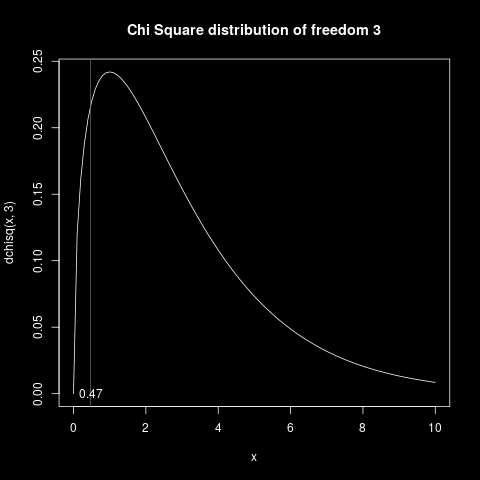
\includegraphics[scale=0.35]{Figure_10-3-4-neg.png}
\end{minipage}

\end{frame}
%-------------- end slide -------------------------------%}}}
%-------------- start slide -------------------------------%{{{ 10.34
\begin{frame}[fragile]

\begin{enumerate}
	\item[E.g. 2'] A second look at the random generator in E.g. 2.\\[1em]
		Does it fit the model too well? Find the $P$-value. \\
\vfill
\begin{minipage}{0.4\textwidth}
\centering
\begin{lstlisting}
> # Example 10.3.1
> x=seq(0,10,0.1)
> plot(x,dchisq(x,2),type = "l")
> abline(v=1.84,col = "gray60")
> text(1.84,0,"1.84")
> title("Chi Square distribution
+       of freedom 2")
> pchisq(1.84,2)
[1] 0.601481
\end{lstlisting}
\end{minipage}
\hfill
\begin{minipage}{0.5\textwidth}
\centering
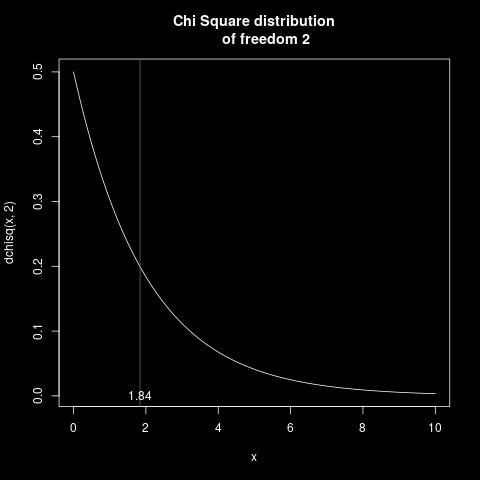
\includegraphics[scale=0.35]{Figure_Example-10-3-1-neg.png}
\end{minipage}
\vfill
\[
	P\text{-value} = 0.601\quad\Longrightarrow \quad \text{No.}
\]
\end{enumerate}
\end{frame}
%-------------- end slide -------------------------------%}}}

\mySection{10.4  Goodness-of-Fit Tests: Parameters Unknown}
%-------------- start slide -------------------------------%{{{ 10.37
\begin{frame}
	% {\S\: 10.4  Goodness-of-Fit Tests: Parameters Unknown}
\begin{center}
\renewcommand{\arraystretch}{2}
\begin{tabular}{c|c}
	$p_i$ are known \cellcolor{gray!50!background}                  & $p_i$ are unknown \cellcolor{gray!50!background}                           \\ \hline
	$D=\sum_{i=1}^t  \frac{\left(X_i-np_i \right)^2}{np_i}$         & $D_1=\sum_{i=1}^t  \frac{\left(X_i-n\hat p_i \right)^2}{n \hat p_i}$       \\
	$\chi^2$ with f.d. $t-1$                                        & $\chi^2$ with f.d. $t-1-s$                                                 \\
	$d=\sum_{i=1}^t  \frac{\left(k_i-n p_{i0} \right)^2}{n p_{i0}}$ & $d_1=\sum_{i=1}^t  \frac{\left(k_i-n\hat p_{i0} \right)^2}{n \hat p_{i0}}$ \\
	$np_{i0}\ge 5$                                                  & $n\hat p_{i0}\ge 5$                                                        \\
	$d>\chi^2_{1-\alpha,t-1}$                                       & $d_1>\chi^2_{1-\alpha,t-1-s}$
\end{tabular}
\end{center}
\vfill
\begin{enumerate}
\item[$\dagger$] $s$ is the number of unknown parameters.\\
\[
\text{df} = \text{\underline{number of classes}} -1 -
\text{\underline{number of unknown parameters.}}
\]
\end{enumerate}
\end{frame}
%-------------- end slide -------------------------------%}}}
%-------------- start slide -------------------------------%{{{ 10.38
\begin{frame}
\begin{enumerate}
\item[E.g. 1] Binomial data:
4096 students, each shots basketball $4$ times.
Let $X_i$ be the number of hits for the $i$th student.
\begin{center}
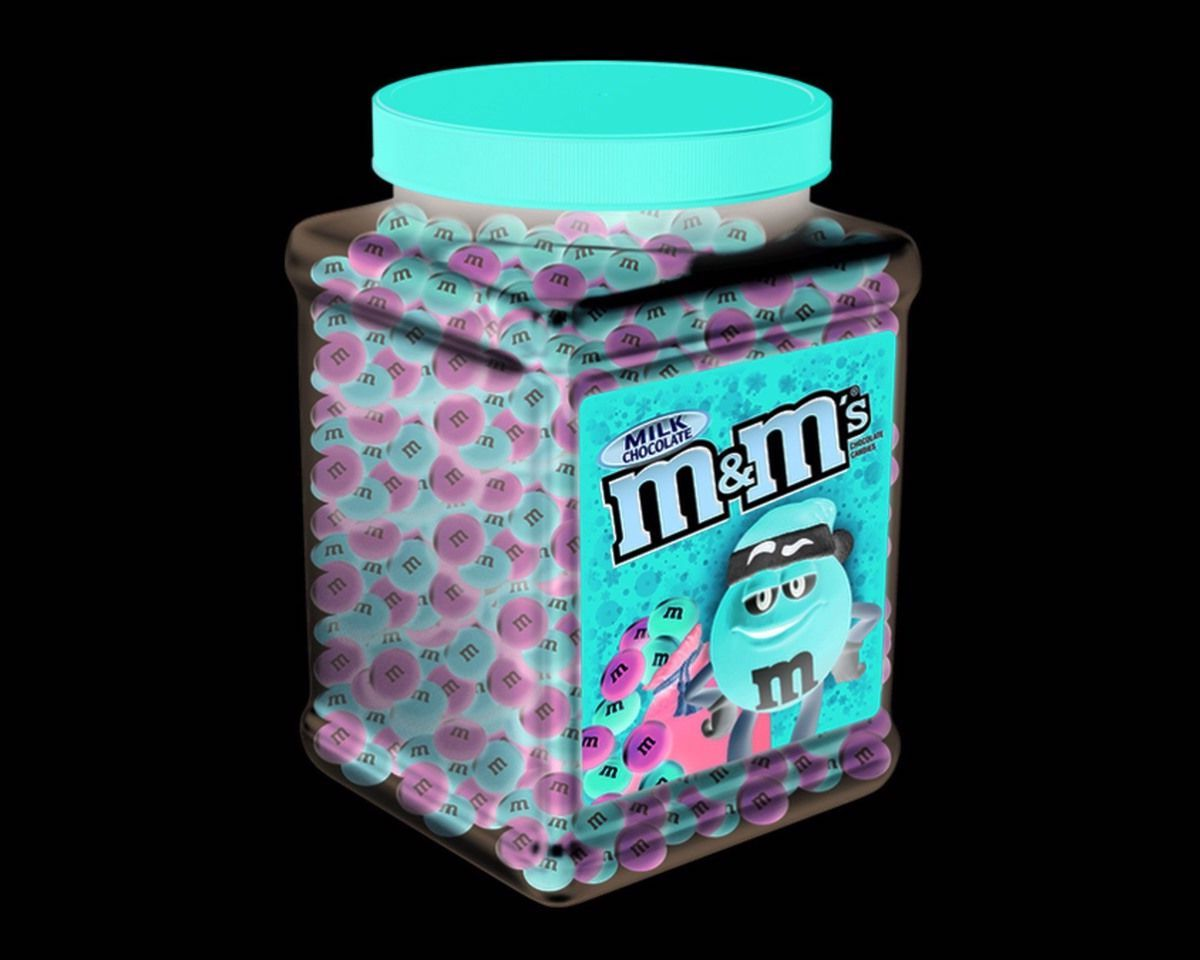
\includegraphics[scale=0.1]{MM_twocolors-neg.jpeg}	\qquad
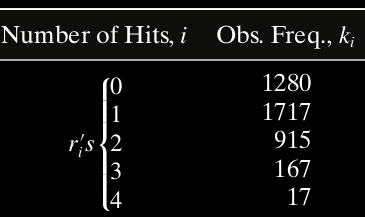
\includegraphics[scale=0.3]{Table_10-4-1-1-neg.png}
\end{center}
\item[] People believe that $X_i$ should following binomial$(4,p)$, that is,
shotting basketball should be something like trying to get red chocolate beans
from a jar of beans of two colors.\\[1em]
\item[] Find the MLE for $p$. Use the data to make a conclusion.
\vfill
\item[Sol.] 1) $H_0:$ $X_i\sim$binomal($4,p$).\\[1em]
\item[] 2) Under $H_0$, the MLE for $p$ is $p_e= ... = 0.251$
\end{enumerate}
\end{frame}
%-------------- end slide -------------------------------%}}}
%-------------- start slide -------------------------------%{{{ 10.39
\begin{frame}

\begin{enumerate}
\item[] 3) Compute the expected frequenies:
\begin{center}
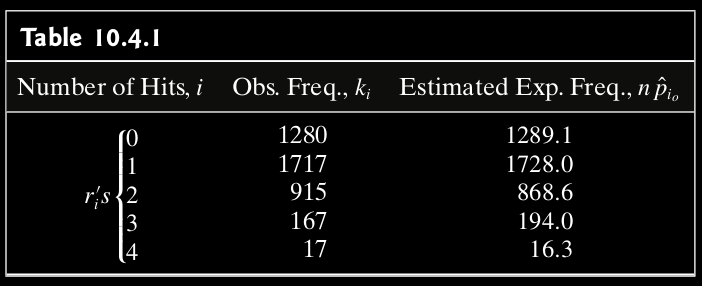
\includegraphics[scale=0.3]{Table_10-4-1-neg.png}
\end{center}
\[
\Longrightarrow\quad			d_1 = \cdots = 6.401.
\]
\vfill
\item[] 4) Critical region: $(\chi^2_{.95,5-1-1},+\infty) =(7.815,+\infty) $
\item[] 5) Conclusion: Fail to reject.
\vfill
\item[] 6) Alternatively, $P$-value $=\bbP(\chi_3^2\ge 6.401) =  0.094$, ... discuss...\myEnd
\end{enumerate}
\end{frame}
%-------------- end slide -------------------------------%}}}
%-------------- start slide -------------------------------%{{{ 10.40
\begin{frame}

\begin{enumerate}
\item[E.g. 2] Does the number of death per day follow the Poisson distribution?
	\vfill
\begin{center}
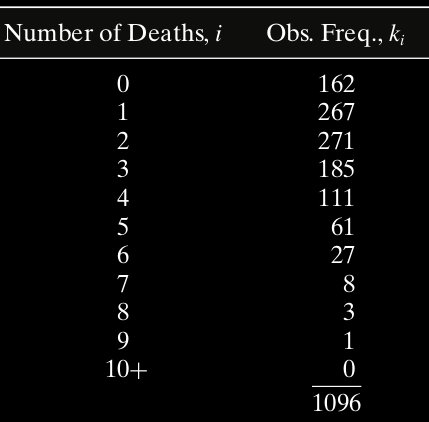
\includegraphics[scale=0.3]{Table_10-4-2-1-neg.png}
\end{center}
\end{enumerate}
\end{frame}
%-------------- end slide -------------------------------%}}}
%-------------- start slide -------------------------------%{{{ 10.41
\begin{frame}
	\begin{enumerate}
		\item[Sol.] 1) Let $X_i$ be the number of death in $i$th day, $1\le i\le 1096$.\\
			\vfill
		\item[] 2) $H_0:$ $X_i$ follow Poisson$(\lambda)$.
			\vfill
		\item[] 3) The MLE for $\lambda$ is: $\lambda_e = \cdots = 2.157$.
			\vfill
		\item[] 4) Compute the expected frequencies:
\begin{center}
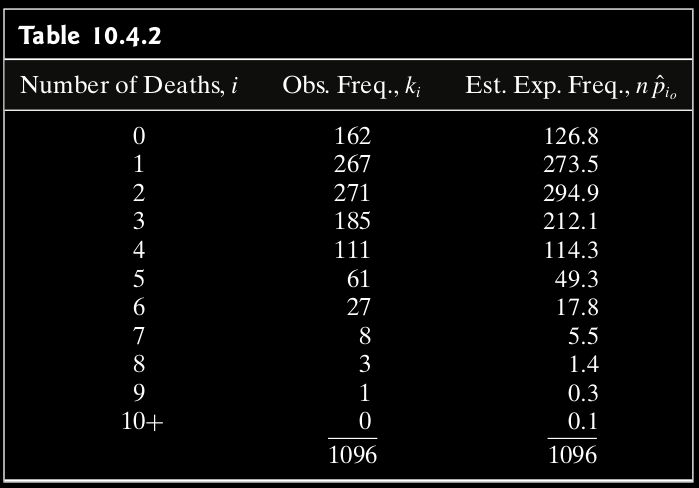
\includegraphics[scale=0.2]{Table_10-4-2-neg.png}
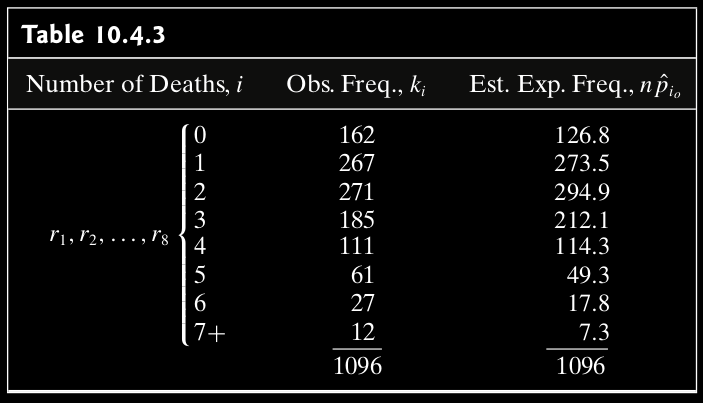
\includegraphics[scale=0.2]{Table_10-4-3-neg.png}
\end{center}
\pause
\[
\Longrightarrow \quad d_1 = \cdots = 25.98.
\]
\vfill
\pause
\item[] 5) $P$-value $= \bbP(\chi_{1,8-1-1}^2\ge 25.98) =0.00022$. Reject! \myEnd
	\end{enumerate}
\end{frame}
%-------------- end slide -------------------------------%}}}

\mySection{10.5 Contingency Tables}
%-------------- start slide -------------------------------%{{{ 10.44
\begin{frame}[2-]
	% {\S\: 10.5 Contingency Tables}
	\begin{enumerate}
		\item[E.g. 1] Whether are the two ratings independent?
			\vfill
			\begin{center}
				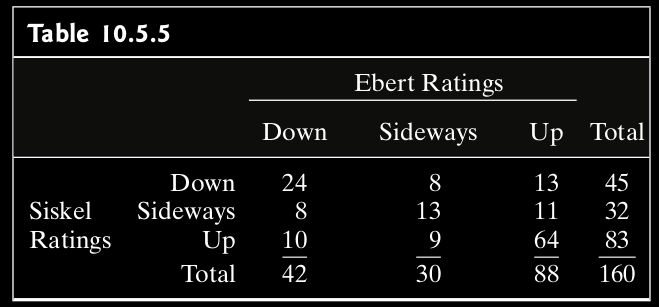
\includegraphics[scale=0.3]{Table_10-5-5-neg.png}
			\end{center}
	\end{enumerate}
\end{frame}
%-------------- end slide -------------------------------%}}}
%-------------- start slide -------------------------------%{{{ 10.45
\begin{frame}[2,4]
	\begin{enumerate}
		\item[E.g. 2] Whether is the suicide rate independent of the mobility factor?
			\vfill
			\begin{center}
				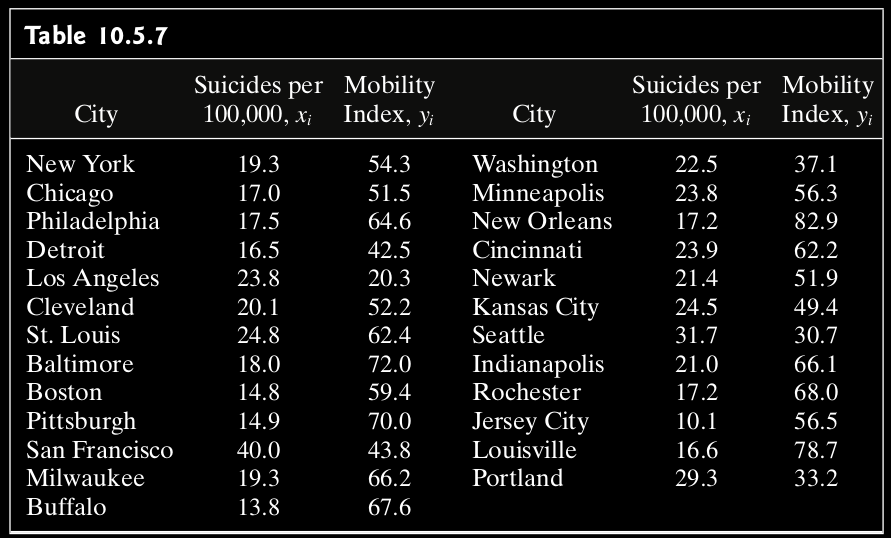
\includegraphics[scale=0.25]{Table_10-5-7-neg.png}
			\end{center}
			\pause
		\item[]\[
				\bar{x} = 20.8\quad\text{and}\quad \bar{y} = 56.0
			\]
			\begin{center}
				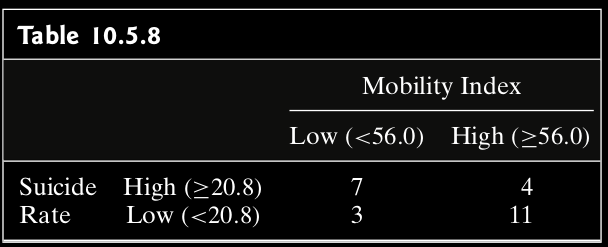
\includegraphics[scale=0.25]{Table_10-5-8-neg.png}
			\end{center}
	\end{enumerate}
\end{frame}
%-------------- end slide -------------------------------%}}}
%-------------- start slide -------------------------------%{{{ 10.46
\begin{frame}
	\begin{enumerate}
		\item[Thm \small 10.4.1] Suppose that $n$ observations are taken on a sample space partitioned by the
			events $A_1,\cdots, A_r$ and $B_1,\cdots,B_c$. \\[1em]
		\item[] Let $p_i=\bbP(A_i)$, $q_j = \bbP(B_j)$, $p_{ij} = \bbP(A_i\cap B_j)$.\\[1em]
		\item[] Let $X_{ij}$ be the number of observations belonging to $A_i\cap B_j$.
			\vfill
		\item[a)] Provided that $np_{ij}\ge 5$ for all $i,j$, the r.v.
			\[
				D_2 = \sum_{i=1}^r \sum_{j=1}^c  \frac{\left(X_{ij}-np_{ij} \right)^2}{np_{ij}} \sim \text{Chi square of f.d. $rc-1$}
			\]
			\vfill
		\item[b)] To test $H_0:$ $A_i$'s are independent of $B_i$'s, calculate the test statistic
			\[
				d_2 = \sum_{i=1}^r \sum_{j=1}^c  \frac{\left(k_{ij}-n\hat p_{i}\hat q_j \right)^2}{n\hat p_{i}\hat q_j}
			\]
			where $\hat p_i$ and $\hat q_j$ are MLE's for $p_i$ and $q_j$, respectively.\\[1em]
		\item[] Provided that $n\hat p_i \hat q_j\ge 5$ for all $i,j$, the critical region is
			\[
				(\chi^2_{1-\alpha,(r-1)(c-1)},+\infty)
			\]
	\end{enumerate}
\end{frame}
%-------------- end slide -------------------------------%}}}
%-------------- start slide -------------------------------%{{{ 10.47
\begin{frame}[2-]

	\begin{enumerate}
		\item[E.g. 1] Sol: Compute the expected frequencies:\\[1em]
			\begin{center}
				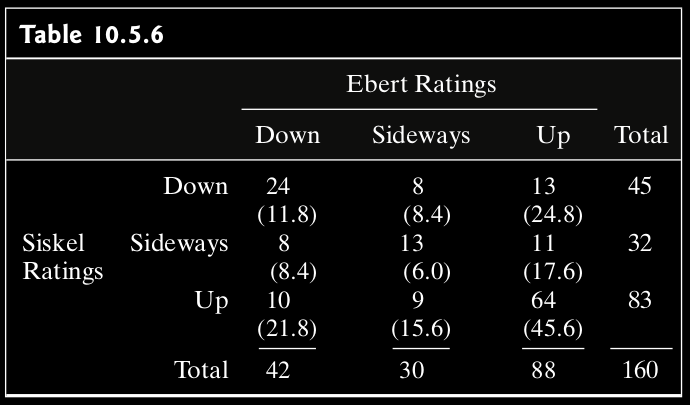
\includegraphics[scale=0.25]{Table_10-5-6-neg.png}
			\end{center}
			\pause
		\item[]
			\[
			\Longrightarrow \quad d_2 = \cdots = 45.37
			\]
			\vfill
		\item[] Critical region is
			\[
				\left(\chi^2_{0.99,(3-1)\times (3-1)},+\infty \right) = (13.277,+\infty)
			\]
		\item[] Alternatively $P$-value = $\bbP(\chi^2_4 \ge 45.37)=   3.33\times 10^{-9}$.
			\vfill
		\item[] Rejection at $\alpha=0.01$.\myEnd
	\end{enumerate}
\end{frame}
%-------------- end slide -------------------------------%}}}
%-------------- start slide -------------------------------%{{{ 10.48
\begin{frame}[2-]

	\begin{enumerate}
		\item[E.g. 2] Sol: Compute the expected frequencies:\\[1em]
			\begin{center}
				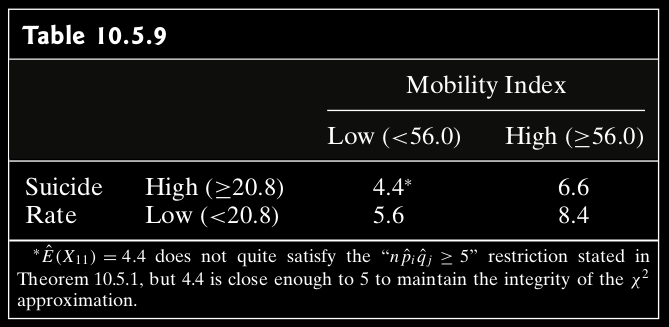
\includegraphics[scale=0.25]{Table_10-5-9-neg.png}
			\end{center}
			\pause
		\item[]
			\[
			\Longrightarrow \quad d_2 = \cdots = 4.57
			\]
			\vfill
		\item[] Critical region is
			\[
				\left(\chi^2_{0.95,(2-1)\times (2-1)},+\infty \right) = (3.41,+\infty)
			\]
		\item[] Alternatively $P$-value = $\bbP(\chi^2_1\ge 4.57)=  0.033$
			\vfill
		\item[] Rejection at $\alpha=0.05$.\myEnd
	\end{enumerate}
\end{frame}
%-------------- end slide -------------------------------%}}}

\end{document}

